\chapter{Foundations for inference}
\label{foundationsForInference}

\section{Variability in estimates}
\label{variabilityInEstimates}

The standard deviation of a sample mean is an important calculation. If the $X_i$ are independent then we can use the fact that for independent $X$, $Y$, $\Var(X+Y)=\Var(X)+\Var(Y)$. So if $\Var(X_i)=\sigma^2$ for all $i$ then
\[
\Var^2\left(\frac1n\sum_{i=1}^nX_i\right) = \frac1{n^2}\sum_{i=1}^n\Var^2(X_i) = \frac1{n^2}\cdot n\cdot\sigma^2 = \sigma^2/n.
\]
Thus the standard deviation of the sample mean is $\sigma/\sqrt{n}$.


\index{point estimate|(}
\index{point estimate!single mean|(}

\begin{figure}%[h]
   \centering
   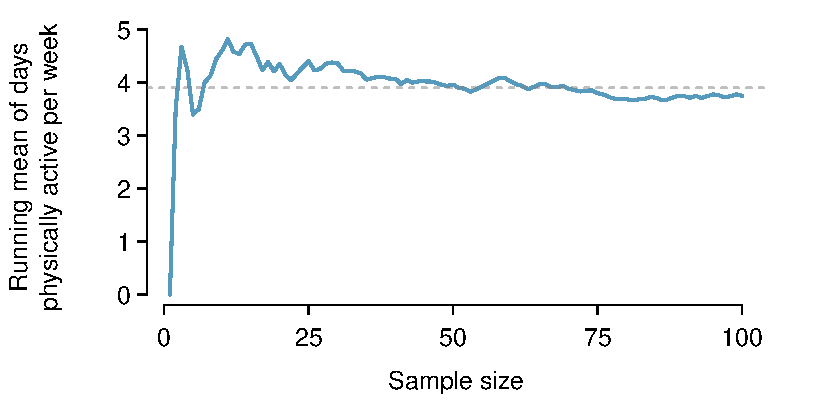
\includegraphics[width=0.72\textwidth]{ch_inference_foundations/figures/yrbssActiveRunningMean/yrbssActiveRunningMean}
   \caption{The mean computed after adding each individual to the sample. The mean tends to approach the true population average as more data become available.}
   \label{yrbssActiveRunningMean}
\end{figure}


Theoretically, the \term{sampling distribution} is the probability distribution of the sample mean of a distribution. In practice, this means that if you observe many (say $m$ many) sample means $\sum_{i=1}^n X_{i,j}/n$, $1\le j\le m$, from a random variable $X$ with a given probability distribution, the observed distribution of these means will be close to the theoretical sampling distribution. Note that these means all have the same value of $n$, and indeed the sampling distribution depends on $n$.

\begin{termBox}{\tBoxTitle{Sampling distribution}
The sampling distribution represents the distribution of the point estimates based on samples of a fixed size from a certain population. It is useful to think of a particular point estimate as being drawn from such a distribution. Understanding the concept of a sampling distribution is central to understanding statistical inference.}
\end{termBox}

The standard deviation of the sample mean is called the \term{standard error (SE)}\index{SE}\marginpar[\raggedright\vspace{-4mm}

$\SE$\\\footnotesize standard\\error]{\raggedright\vspace{-4mm}

$\SE$\\\footnotesize standard\\error} of the estimate.

\begin{termBox}{\tBoxTitle{Standard error of an estimate}
The standard deviation associated with an estimate is called the \emph{standard error}. It describes the typical error or uncertainty associated with the estimate.}
\end{termBox}




\begin{termBox}{\tBoxTitle{Computing SE for the sample mean}
Given $n$ independent observations from a population with standard deviation $\sigma$, the standard error of the sample mean is equal to \vspace{-1mm}
\begin{eqnarray}
\SE = \frac{\sigma}{\sqrt{n}}
\label{seOfXBar}
\end{eqnarray}\vspace{-3mm}%

A reliable method to ensure sample observations are independent is to conduct a simple random sample consisting of less than 10\% of the population.\index{standard error (SE)!single mean}
}
\end{termBox}


\begin{example}{Standard example}%Thanks to Daniel T.
Suppose you have two Bernoulli random variables $X$ and $Y$ that are independent and have the same parameter $p$.
We can use $\frac{X+Y}2$ as our estimate of $p$. This will tend to be closer to $p$ than if we only used $X$. For one thing, $X$ can only take the values 0 and 1,
whereas $\frac{X+Y}2$ can also take the value $1/2$. In this case $\sigma=\sqrt{p(1-p)}$ and the standard error is $\sqrt{p(1-p)/2}$.
Of course, if we don't know what $p$ is then we don't know this standard error, either, so we use $\SE=\sqrt{\hat p(1-\hat p)/n}$ instead, where $\hat p =\frac{X+Y}2$.
For small $n$ like $n=2$ here, this SE may be zero, so we should not divide by it. For large $n$ and moderate $0<p<1$, however, this will not be a problem.
\end{example}



\index{point estimate|)}


%__________________
\section{Confidence intervals}
\label{confidenceIntervals}

\index{confidence interval|(}

A point estimate provides a single plausible value for a parameter. However, a point estimate is rarely perfect; usually there is some error in the estimate. Instead of supplying just a point estimate of a parameter, a next logical step would be to provide a plausible \emph{range of values} for the parameter.


A plausible range of values for the population parameter is called a \term{confidence interval}.

\subsection{Confidence interval for the exponential distribution}
Suppose $X$ is a random variable that is exponentially distributed with parameter $\lambda$, so that $f_X(x)=\lambda e^{-\lambda x}$.
Given one observation, what can we say about $\lambda$?
Notice that $Y=\lambda X$ is exponentially distributed with parameter 1, since
\[
f_Y(y) = \frac{d}{dy}\mathbb P(Y \le y) = \frac{d}{dy}\mathbb P(\lambda X \le y) = \frac{d}{dy}F_X(y/\lambda) = \frac1{\lambda} f_X(y/\lambda)
= e^{-y}.
\]
In order to obtain a 90\% confidence interval we choose $y_0, y_1$ such that $1-e^{-y_0}=\mathbb P(Y\le y_0)=5\%=\mathbb P(Y\ge y_1)=e^{-y_1}$.
Thus, $y_0=\ln 20 - \ln 19 = 0.051$. (Notice that $y_0\approx 5\%$; this is because $e^{-x}\approx 1-x$ for small positive $x$.)
Similarly, $y_1 = \ln 20 = 2.9957$. (It is a somewhat famous fact that $e^3\approx 20$.)
Now we have
\[
90\% = \mathbb P(y_0 \le Y \le y_1) = \mathbb P(y_0 \le \lambda X \le y_1) = \mathbb P(y_0/X \le \lambda \le y_1/X) = \mathbb P(\lambda\in [y_0/X,y_1/X]).
\]
Now I'll secretly choose a value for $\lambda$ and draw some random values:
\begin{equation}\label{eq:values}
X(\omega_1) = 0.231,\quad X(\omega_2) = 0.6324,\quad X(\omega_3) = 0.03144.
\end{equation}
This can be done by first picking $r$ uniformly from the unit interval $[0,1]$, and then letting $x$ be such that $\mathbb P(X \le x) = r$, and reporting $x$ as the value of $X$.

The interval $[y_0/x,y_1/x]$ is then a 90\% confidence interval for $\lambda$.
For our particular values, the interval is
\[
\left[,\frac{0.051}{0.231}, \frac{2.9957}{0.231} \right] = \left[ 0.22, 13.03\right].
\]
For the other two values in \eqref{eq:values} the intervals are $[0.08, 4.74]$ and $[1.62, 95.3]$ (exercise: verify this).
What is a value for $\lambda$ that lies in all of these intervals? In October 2025 a student guessed $\lambda=3$ and indeed, that is
the value of $\lambda$ I had used. The fact that the correct value was in all the three confidence intervals is not something that will always happen,
in fact the probability of it happening is $90\%^3 = 72.9\%$.

The subtle and key point to observe here is that the confidence interval is random: it depends on the value of the random variable $X$.
The parameter $\lambda$ is not random; it is constant, but unknown.

\subsection{Normal distribution}
\begin{termBox}{\tBoxTitle{Central Limit Theorem, informal description}
If a sample consists of at least 30 independent observations and the data are not strongly skewed, then the distribution of the sample mean is well approximated by a~normal model.\index{Central Limit Theorem}}
\end{termBox}

\index{confidence interval!confidence level|(}



\begin{figure}%[h]
\centering
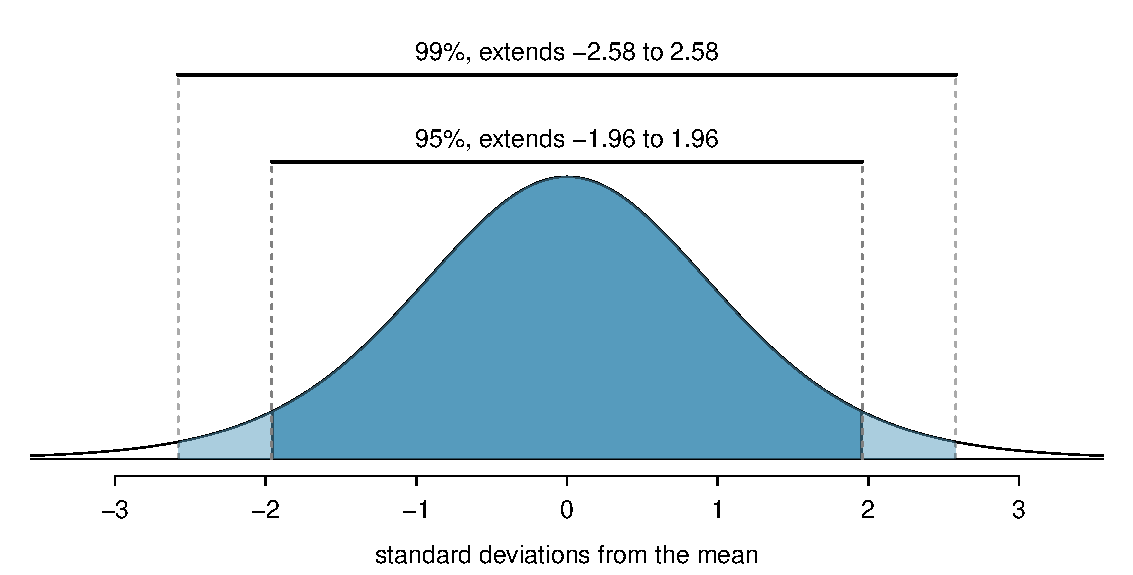
\includegraphics[width=\textwidth]{ch_inference_foundations/figures/choosingZForCI/choosingZForCI}
\caption{The area between -$z^{\star}$ and $z^{\star}$ increases as $|z^{\star}|$ becomes larger. If the confidence level is 99\%, we choose $z^{\star}$ such that 99\% of the normal curve is between -$z^{\star}$ and $z^{\star}$, which corresponds to 0.5\% in the lower tail and 0.5\% in the upper tail: $z^{\star}=2.58$.}
\label{choosingZForCI}
\index{confidence interval!confidence level|)}
\end{figure}

The normal approximation is crucial to the precision of these confidence intervals. Section~\ref{cltSection} provides a more detailed discussion about when the normal model can safely be applied. When the normal model is not a good fit, we will use alternative distributions that better characterize the sampling distribution.

\begin{termBox}{\tBoxTitle{Conditions for $\bar{x}$ being nearly normal and $\SE$ being accurate\label{terBoxOfCondForXBarBeingNearlyNormalAndSEBeingAccurate}}
Important conditions to help ensure the sampling distribution of $\bar{x}$ is nearly normal and the estimate of SE sufficiently accurate:
\begin{itemize}
\setlength{\itemsep}{0mm}
\item The sample observations are independent.
\item The sample size is large: $n\geq30$ is a common rule of thumb.
\item The population distribution is itself not too different from the normal distribution in terms of skew.
\end{itemize}
Additionally, the larger the sample size, the more lenient we can be with the sample's skew.}
\end{termBox}

\begin{tipBox}{\tipBoxTitle[]{How to verify sample observations are independent}
If the observations are from a simple random sample and consist of fewer than 10\% of the population, then they may be considered to be approximately independent.\\[2mm]
Subjects in an experiment are considered independent if they undergo random assignment to the treatment groups. \\[2mm]
If a sample is from a seemingly random process, e.g. the lifetimes of wrenches used in a particular manufacturing process, checking independence is more difficult. In~this case, use your best judgement.}
\end{tipBox}


It is too much to ask but it may be worth remembering that 99\% confidence corresponds to 2.58 standard deviations and 90\% to 1.65.


\begin{termBox}{\tBoxTitle{Confidence interval for any confidence level}
If the point estimate follows the normal model with standard error $\SE$, then a confidence interval for the population parameter is
\begin{eqnarray*}
\text{point estimate}\ \pm\ z^{\star} \SE
\end{eqnarray*}
where $z^{\star}$ corresponds to the confidence level selected.}
\end{termBox}

Figure~\ref{choosingZForCI} provides a picture of how to identify $z^{\star}$ based on a confidence level. We~select $z^{\star}$ so that the area between -$z^{\star}$ and $z^{\star}$ in the normal model corresponds to the confidence level. That is, if the area is 95\%, say, then we have 95\% confidence.

\begin{termBox}{\tBoxTitle{Margin of error}
\label{marginOfErrorTermBox}In a confidence interval, $z^{\star}\times \SE$ is called the \term{margin of error}.}
\end{termBox}

\index{confidence interval!interpretation|(}
\index{confidence interval!interpretation|)}
\index{confidence interval|)}

\subsection{Election polls}\label{oct-24-2025}
Alice and Bob are running for Mayor of Honolulu.
In a simple random sample of $n=1000$ voters, Alice had the support of 510 and Bob of 490.
Does this give us confidence that Alice will win?
Let $X$ be a binomial random variable with parameters $n=1000$ and $p$ being the unknown support that Alice has
in the population at large. Since Honolulu has around 1 million voters, it is reasonable to model using a binomial distribution.
The mean of $X$ is $np$ and the standard deviation $\sigma(X)$ is $\sqrt{np(1-p)}$. Since $p$ is unknown, we approximate the standard deviation by $\sqrt{n}/2$, using $p\approx 1/2$. (To be a bit more precise we can use $p\approx \frac{510}{1000}$.)
Now $X$ is approximately normal by the Central Limit Theorem, so if we let 
\[
Z = \frac{X - \mathbb E(X)}{\sigma(X)}
\]
then $Z$ is approximately standard normal, so that
\[
95\% \approx \mathbb P(|Z|\le 2).
\]
Note that $\sigma(X)\approx \sqrt{1000}/2=5\sqrt{10}<16$ (since upon squaring both sides, $250<256$)
so $2\sigma(X)<32$.
The statement that we have 95\% confidence in is that $-2\sigma(X) \le X-1000p \le 2\sigma(X)$,
which has several equivalent forms:
\[-2\sigma(X) \le 1000p-X \le 2\sigma(X)\]
\[X-2\sigma(X) \le 1000p \le X+2\sigma(X)\]
\[\frac{X-2\sigma(X)}{1000} \le p \le \frac{X+2\sigma(X)}{1000}\]
\[\frac{510-2\sigma(X)}{1000} \le p \le \frac{X+2\sigma(X)}{1000}\]
We are if anything \emph{more} confident that $p$ belongs to the wider interval
\[\frac{510-32}{1000} \le p \le \frac{X+32}{1000}\]
In other words $p \in [0.478, 0.542]$. This interval includes some values of $p$ for which Alice loses the election ($p<0.5$)
so we cannot say with 95\% confidence that she will win.
%__________________
\section{Hypothesis testing}
\label{hypothesisTesting}



If the null hypothesis asserts that $p=1/2$ then it is making a very bold assertion. Even if $p=0.500000001$, the null hypothesis is strictly speaking false. This is why we do not "accept" null hypotheses; we cannot gather enough evidence to conclude an assertion with infinite precision. In this setting, a Type 1 error amounts to declaring that $p$ is not $1/2$ when actually it is, which is offensive since $p$ took the trouble to have infinitely many digits correct! A type 2 error is to believe that $p=1/2$ when it's not, so maybe actually $p=0.500000001$. This is potentially not so offensive.

\index{hypothesis testing|(}


\begin{termBox}{\tBoxTitle{Null and alternative hypotheses}
{\small The \term{null hypothesis ($H_0$)} often represents either a skeptical perspective or a claim to be tested. The \term{alternative hypothesis ($H_A$)} represents an alternative claim under consideration and is often represented by a range of possible parameter values.}}
\end{termBox}

The null hypothesis often represents a skeptical position or a perspective of no difference. The alternative hypothesis often represents a new perspective, such as the possibility that there has been a change. 


Note that the main text uses \emph{sample standard deviation} to refer to the standard deviation of the original distribution; so this is not the same as the standard deviation of the sample \emph{mean}, which is also called the standard error.


\subsection{Decision errors}

\index{hypothesis testing!decision errors|(}

\begin{table}%[ht]
\centering
\begin{tabular}{l l c c}
& & \multicolumn{2}{c}{\textbf{Test conclusion}} \\
  \cline{3-4}
\vspace{-3.7mm} \\
& & do not reject $H_0$ &  reject $H_0$ in favor of $H_A$ \\
  \cline{2-4}
\vspace{-3.7mm} \\
& $H_0$ true & No error &  Type~1 Error \\
\raisebox{1.5ex}{\textbf{Truth}} & $H_A$ true & Type~2 Error & No error \\
  \cline{2-4}
\end{tabular}
\caption{Four different scenarios for hypothesis tests.}
\label{fourHTScenarios}
\end{table}

A \term{Type~1 Error} is rejecting the null hypothesis when $H_0$ is actually true. A \term{Type~2 Error} is failing to reject the null hypothesis when the alternative is actually true.


\index{hypothesis testing!decision errors|)}

If we reduce how often we make one type of error, we generally make more of the other type.

Hypothesis testing is built around rejecting or failing to reject the null hypothesis. That is, we do not reject $H_0$ unless we have strong evidence. But what precisely does \emph{strong evidence} mean? As a general rule of thumb, for those cases where the null hypothesis is actually true, we do not want to incorrectly reject $H_0$ more than 5\% of the time. This corresponds to a \term{significance level}\index{hypothesis testing!significance level} of 0.05. We often write the significance level using $\alpha$\marginpar[\raggedright\vspace{-4mm}

$\alpha$\\\footnotesize significance\\level of a\\hypothesis test]{\raggedright\vspace{-4mm}

$\alpha$\\\footnotesize significance\\level of a\\hypothesis test} (the Greek letter \emph{alpha}\index{Greek!alpha@alpha ($\alpha$)}): $\alpha = 0.05$. We discuss the appropriateness of different significance levels in Section~\ref{significanceLevel}.

If we use a 95\% confidence interval to evaluate a hypothesis test where the null hypothesis is true, we will make an error whenever the point estimate is at least 1.96 standard errors away from the population parameter. This happens about 5\% of the time (2.5\% in each tail). Similarly, using a 99\% confidence interval to evaluate a hypothesis is equivalent to a significance level of $\alpha = 0.01$.

A confidence interval is, in one sense, simplistic in the world of hypothesis tests. Consider the following two scenarios:
\begin{itemize}
\setlength{\itemsep}{0mm}
\item The null value (the parameter value under the null hypothesis) is in the 95\% confidence interval but just barely, so we would not reject $H_0$. However, we might like to somehow say, quantitatively, that it was a close decision.
\item The null value is very far outside of the interval, so we reject $H_0$. However, we want to communicate that, not only did we reject the null hypothesis, but it wasn't even close. Such a case is depicted in Figure~\ref{whyWeWantPValue}.
\end{itemize}
In Section~\ref{pValue}, we introduce a tool called the \emph{p-value} that will be helpful in these cases. The p-value method also extends to hypothesis tests where confidence intervals cannot be easily constructed or applied.

\begin{figure}%[hht]
\centering
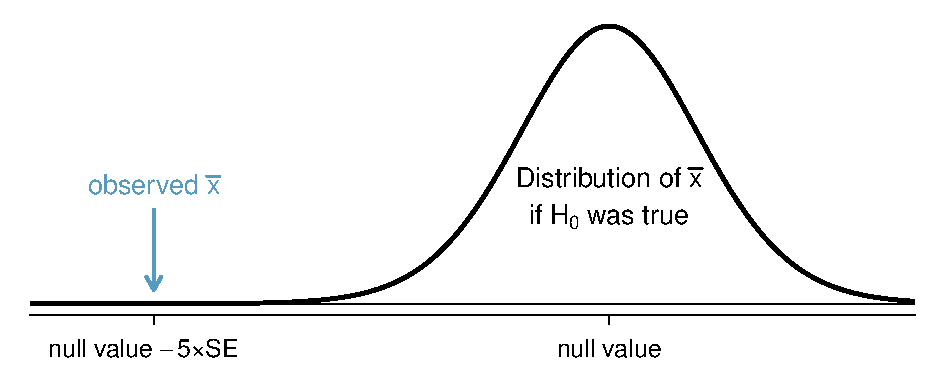
\includegraphics[width=0.75\textwidth]{ch_inference_foundations/figures/whyWeWantPValue/whyWeWantPValue}
\caption{It would be helpful to quantify the strength of the evidence against the null hypothesis. In this case, the evidence is extremely strong.}
\label{whyWeWantPValue}
\end{figure}


\subsection{Formal testing using p-values}
\label{pValue}

\index{hypothesis testing!p-value|(}

The p-value is a way of quantifying the strength of the evidence against the null hypothesis and in favor of the alternative. Formally the \emph{p-value} is a conditional probability.

\begin{termBox}{\tBoxTitle{p-value}
The \term{p-value}\index{hypothesis testing!p-value|textbf} is the probability of observing data at least as favorable to the alternative hypothesis as our current data set, if the null hypothesis is true. We typically use a summary statistic of the data, in this chapter the sample mean, to help compute the p-value and evaluate the hypotheses.}
\end{termBox}


\begin{tipBox}{\tipBoxTitle{Always write the null hypothesis as an equality}
We will find it most useful if we always list the null hypothesis as an equality, like:
\[
H_0: \quad\mu = 7
\]
while the alternative always uses an inequality, like one of the following:
\begin{eqnarray*}
H_A:& \mu\neq7,\quad\text{2-sided},\\
H_A:& \mu>7,\quad\text{1-sided},\\
H_A:& \mu<7,\quad\text{1-sided}.
\end{eqnarray*}
}
\end{tipBox}

\begin{figure}%[hht]
   \centering
   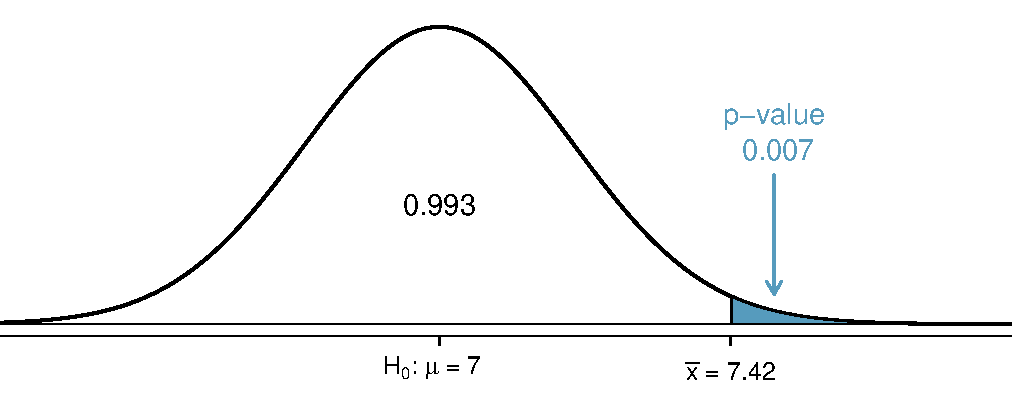
\includegraphics[width=0.83\textwidth]{ch_inference_foundations/figures/pValueOneSidedSleepStudy/pValueOneSidedSleepStudy}
   \caption{Example of $p$-value for a 1-sided hypothesis test.}
   \label{pValueOneSidedSleepStudy}
\end{figure}

The $p$-value is the probability, according to $H_0$, of observing something at least as favorable to $H_A$ as what was actually observed.

If the $p$-value is less than the significance level (say $p$-value $=0.007 < 0.05=\alpha$), we reject the null hypothesis.

\begin{termBox}{\tBoxTitle{p-value as a tool in hypothesis testing}
The smaller the p-value, the stronger the data favor $H_A$ over $H_0$. A small p-value (usually $<0.05$) corresponds to sufficient evidence to reject $H_0$ in favor of $H_A$.}
\index{hypothesis testing!p-value|)}
\end{termBox}


\begin{figure}%[ht]
   \centering
   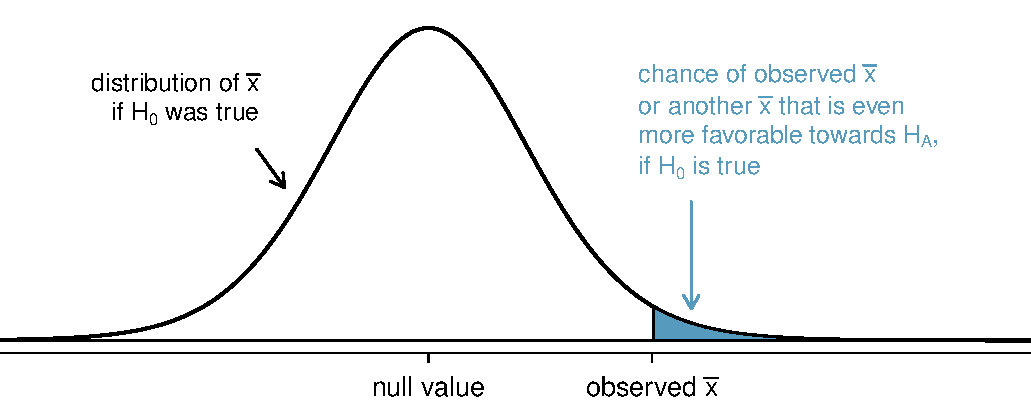
\includegraphics[width=0.9\textwidth]{ch_inference_foundations/figures/pValueOneSidedSleepStudyExplained/pValueOneSidedSleepStudyExplained}
   \caption{To identify the p-value, the distribution of the sample mean is considered as if the null hypothesis was true. Then the p-value is defined and computed as the probability of the observed $\bar{x}$ or an $\bar{x}$ even more favorable to $H_A$ under this distribution.}
   \label{pValueOneSidedSleepStudyExplained}
\end{figure}

\begin{termBox}{\tBoxTitle{What's so special about 0.05?}
The main text gives a video that doesn't really explain it. In fact, we can think of two reasons for $0.05$: it's approximately 2 standard deviations (1.96) and Fisher suggested using 0.05, about a hundred years ago.}
\end{termBox}


\subsection{Two-sided hypothesis testing with p-values}
\label{twoSidedTestsWithPValues}


To compute a $p$-value for a two-sided test, consider Figure \ref{2ndSchSleepHTExample}.
\begin{figure}
   \centering
   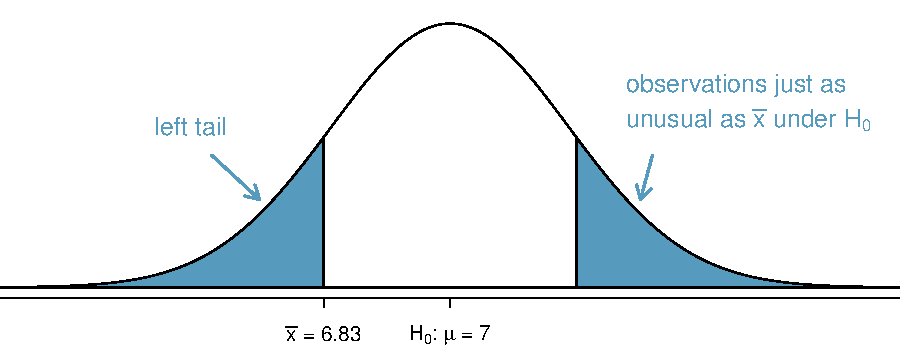
\includegraphics[width=0.9\textwidth]{ch_inference_foundations/figures/2ndSchSleepHTExample/2ndSchSleepHTExample}
   \caption{$H_A$ is two-sided, so \emph{both} tails must be counted for the p-value.}
   \label{2ndSchSleepHTExample}
\end{figure}



\begin{caution}{One-sided hypotheses are allowed only \emph{before} seeing data}
{After observing data, it is tempting to turn a two-sided test into a one-sided test. Avoid this temptation. Hypotheses must be set up \emph{before} observing the data. If~they are not, the test should be two-sided.}
\end{caution}


\subsection{Choosing a significance level}
\label{significanceLevel}

\index{hypothesis testing!significance level|(}
\index{significance level|(}

Choosing a significance level for a test is important in many contexts, and the traditional level is 0.05. However, it is often helpful to adjust the significance level based on the application. We may select a level that is smaller or larger than 0.05 depending on the consequences of any conclusions reached from the test.

If making a Type~1 Error is dangerous or especially costly, we should choose a small significance level (e.g. 0.01). Under this scenario we want to be very cautious about rejecting the null hypothesis, so we demand very strong evidence favoring $H_A$ before we would reject $H_0$.

If a Type~2 Error is relatively more dangerous or much more costly than a Type~1 Error, then we should choose a higher significance level (e.g. 0.10). Here we want to be cautious about failing to reject $H_0$ when the null is actually false.


\index{significance level|)}
\index{hypothesis testing!significance level|)}
\index{hypothesis testing|)}




%__________________
\section{Examining the Central Limit Theorem}
\label{cltSection}

\index{Central Limit Theorem|(}


The \emph{OpenIntro} text gives an informal statement of the CLT. Here we shall not be so advanced as to prove the CLT; but we shall give a precise statement of it.

The CDF of the standardized sample mean $(\overline X-\mu)/\sigma$ of an IID sequence $X_i$ with $\E(X_i)<\infty$ and $\E(X^2)<\infty$ converges pointwise to the CDF of the standard normal distribution.

So
\[
	\lim_{n\to\infty} \P((\overline X_n-\mu)/\sigma\le z) = \Phi(z)
\]
where
\[
	\Phi(z)=\P(Z\le z)=\frac1{\sqrt{2\pi}}\int_{-\infty}^z e^{-z^2/2}\,dz.
\]

The normal model for the sample mean tends to be very good when the sample consists of at least 30 independent observations and the population data are not strongly skewed. The Central Limit Theorem provides the theory that allows us to make this assumption.

\begin{termBox}{\tBoxTitle{Central Limit Theorem, informal definition}
The distribution of $\bar{x}$ is approximately normal. The approximation can be poor if the sample size is small, but it improves with larger sample sizes.}
\end{termBox}

The Central Limit Theorem states that when the sample size is small, the normal approximation may not be very good. However, as the sample size becomes large, the normal approximation improves. We will investigate three cases to see roughly when the approximation is reasonable.

We consider three data sets: one from a \emph{uniform} distribution, one from an \emph{exponential} distribution, and the other from a \emph{log-normal} distribution. These distributions are shown in the top panels of Figure~\ref{cltSimulations}. The uniform distribution is symmetric, the exponential distribution may be considered as having moderate skew since its right tail is relatively short (few outliers), and the log-normal distribution is strongly skewed and will tend to produce more apparent outliers.\index{skew!example: moderate}\index{skew!example: strong}

\begin{figure}
   \centering
   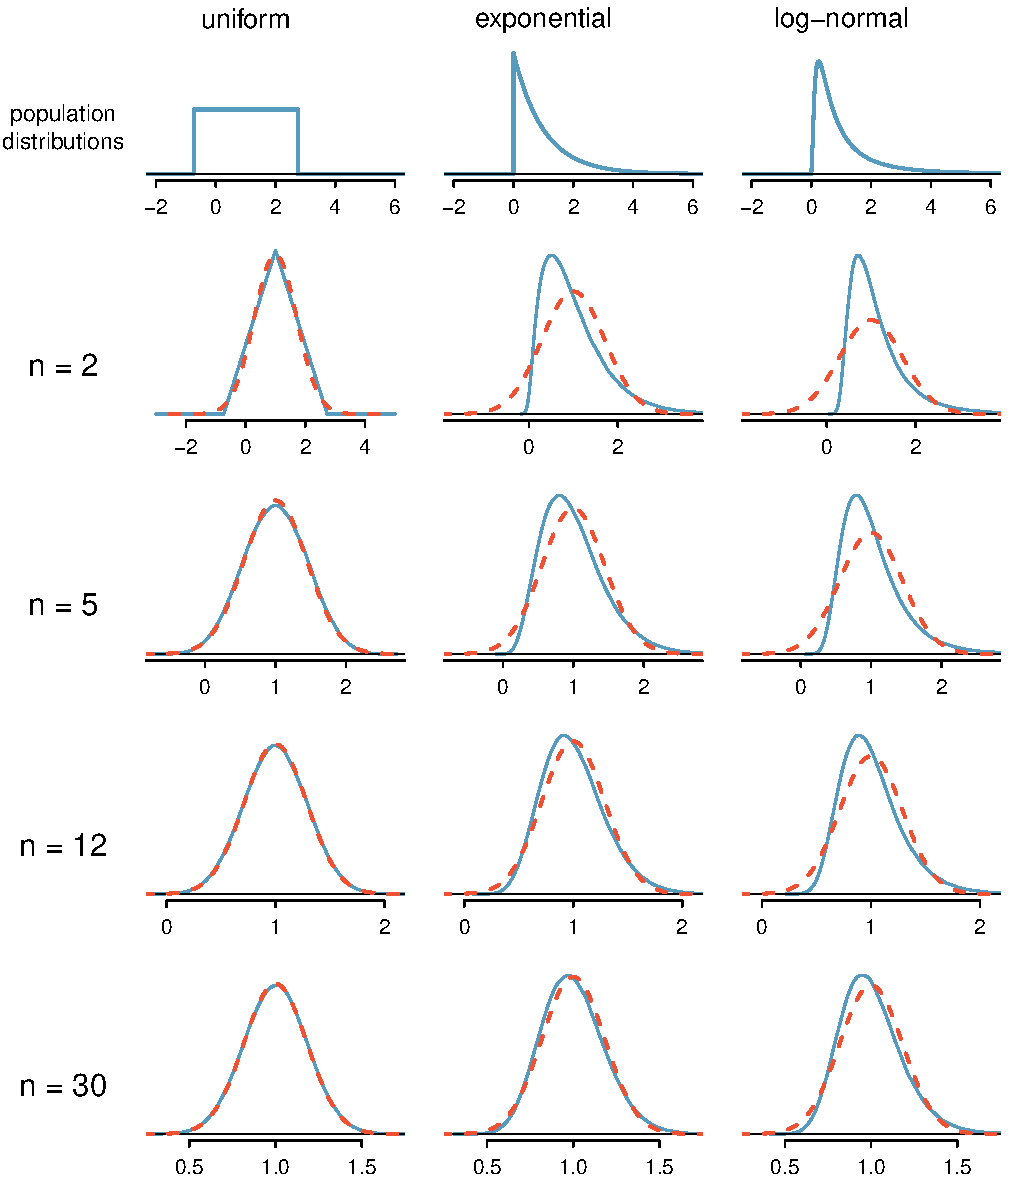
\includegraphics[width=\textwidth]{ch_inference_foundations/figures/cltSimulations/cltSimulations}
   \caption{Sampling distributions for the mean at different sample sizes and for three different distributions. The dashed red lines show normal distributions.}
   \label{cltSimulations}
\end{figure}

The left panel in the $n=2$ row represents the sampling distribution of $\bar{x}$ if it is the sample mean of two observations from the uniform distribution shown. The dashed line represents the closest approximation of the normal distribution. Similarly, the center and right panels of the $n=2$ row represent the respective distributions of $\bar{x}$ for data from exponential and log-normal distributions.

\begin{example}{Would the normal approximation be good in all applications where the sample size is at least 30?}
Not necessarily. For example, the normal approximation for the log-normal example is questionable for a sample size of 30. Generally, the more skewed a population distribution or the more common the frequency of outliers, the larger the sample required to guarantee the distribution of the sample mean is nearly normal.
\end{example}

\begin{caution}
{Examine data structure when considering independence}
{Some data sets are collected in such a way that they have a natural underlying structure between observations, e.g. when observations occur consecutively. Be especially cautious about independence assumptions regarding such data sets.}
\end{caution}

\begin{caution}{Watch out for strong skew and outliers}
{Strong skew is often identified by the presence of clear outliers. If a data set has prominent outliers, or such observations are somewhat common for the type of data under study, then it is useful to collect a sample with many more than 30 observations if the normal model will be used for $\bar{x}$.}
\index{Central Limit Theorem|)}
\end{caution}

\index{skew!strongly skewed guideline}


\subsection{Exponential, log-normal, uniform}
We explain the distributions in Figure \ref{cltSimulations}.

The \term{exponential distribution} with parameter $\lambda$ is an important distribution omitted in \emph{OpenIntro}. It is the continuous-time analogue of the geometric distribution. It has pdf
\[
	f_X(x)=\lambda\cdot e^{-\lambda x},\quad 0\le x<\infty.
\]
You can verify that it has a memory-less property shared with the geometric distribution, namely
\[
	\P(X\ge x+y\mid X\ge x) = \P(X\ge y).
\]
The \term{log-normal} distribution is important in finance. It can be used to model stock prices, which are always nonnegative.
\begin{df}\label{lognormal}
$X$ is a log-normal random variable with parameters $\mu$ and $\sigma$ if $X=e^W$ where the logarithm $W$ is normal with parameters $\mu$ and $\sigma$.
\end{df}

The \term{uniform} distribution on an interval $[a,b]$ has a constant pdf on that interval:
\[
	f_X(x)=\frac1{b-a},\quad a\le x\le b.
\]



%__________________
\section{Inference for other estimators}
\label{aFrameworkForInference}

The sample mean is not the only point estimate for which the sampling distribution is nearly normal. For example, the sampling distribution of sample proportions closely resembles the normal distribution when the sample size is sufficiently large. In this section, we introduce a number of examples where the normal approximation is reasonable for the point estimate. Chapters~\ref{inferenceForNumericalData} and~\ref{inferenceForCategoricalData} will revisit each of the point estimates you see in this section along with some other new statistics.

We make another important assumption about each point estimate encountered in this section: the estimate is unbiased. A point estimate is \term{unbiased} if the sampling distribution of the estimate is centered at the parameter it estimates. That is, an unbiased estimate does not naturally over or underestimate the parameter. Rather, it tends to provide a ``good'' estimate. The sample mean is an example of an unbiased point estimate, as are each of the examples we introduce in this section.

Finally, we will discuss the general case where a point estimate may follow some distribution other than the normal distribution. We also provide guidance about how to handle scenarios where the statistical techniques you are familiar with are insufficient for the problem at hand.


\subsection{Confidence intervals for nearly normal point estimates}

\index{confidence interval!using normal model|(}

In Section~\ref{confidenceIntervals}, we used the point estimate $\bar{x}$ with a standard error $\SE_{\bar{x}}$ to create a 95\% confidence interval for the population mean:
\begin{align}
\bar{x}\ \pm\ 1.96 \times \SE_{\bar{x}}
\label{95PercCIForMeanInGeneralizingSection}
\end{align}
We constructed this interval by noting that the sample mean is within 1.96 standard errors of the actual mean about 95\% of the time. This same logic generalizes to any unbiased point estimate that is nearly normal. We may also generalize the confidence level by using a place-holder $z^{\star}$.

\begin{termBox}{\tBoxTitle{General confidence interval for the normal sampling distribution case}\label{generalConfidenceIntervalTermBox}%
A confidence interval based on an unbiased and nearly normal point estimate is
\begin{eqnarray}
\text{point estimate}\ \pm\ z^{\star}\SE
\label{95PercGeneralCIInGeneralizingSection}
\end{eqnarray}
where $z^{\star}$ is selected to correspond to the confidence level, and $\SE$ represents the standard error. The value $z^{\star}\SE$ is called the \emph{margin of error}\index{margin of error}.}
\end{termBox}

Generally the standard error for a point estimate is estimated from the data and computed using a formula. For example, the standard error for the sample mean is
\begin{eqnarray*}
\SE_{\bar{x}} = \frac{s}{\sqrt{n}}
\end{eqnarray*}

%Thanks to Keanu:
The variance of a sample mean $\sum_{i=1}^n X_i/n$, where the $X_i$ are iid with variance $\sigma^2$, is $\sigma^2/n$, by the following calculation (which uses the fact, proved in advanced courses, that the variance of a sum of independent random variables is the sum of their variances):
\begin{eqnarray*}
	\Var\left(\frac1n\sum_{i=1}^n X_i\right) &=& \frac1{n^2}\Var\left(\sum_{i=1}^n X_i\right)\\
	 &=& \frac1{n^2}\sum_{i=1}^n\Var(X_i)\\
	 &=& \frac{n}{n^2}\Var(X_1) = \frac{\sigma^2}n.
\end{eqnarray*}
Consequently, the standard deviation of the sample mean is $\sigma/\sqrt{n}$. When $\sigma$ is unknown we approximate it by $s$, and hence our estimated standard deviation of the sample mean (the standard error of the mean) is $s/\sqrt{n}$.



\subsection{Hypothesis testing for nearly normal point estimates}
\index{hypothesis testing!using normal model|(}

Just as the confidence interval method works with many other point estimates, we can generalize our hypothesis testing methods to new point estimates. Here we only consider the p-value approach, introduced in Section~\ref{pValue}, since it is the most commonly used technique and also extends to non-normal cases.

\begin{termBox}{\tBoxTitle[]{Hypothesis testing using the normal model}
	\begin{enumerate}
		\setlength{\itemsep}{0mm}
		\item First write the hypotheses in plain language, then set them up in mathematical notation.
		\item Identify an appropriate point estimate of the parameter of interest.
		\item Verify conditions to ensure the standard error estimate is reasonable and the point estimate is nearly normal and unbiased.
		\item Compute the standard error. Draw a picture depicting the distribution of the estimate under the idea that $H_0$ is true. Shade areas representing the p-value.
		\item Using the picture and normal model, compute the \emph{test statistic} (Z-score) and identify the p-value to evaluate the hypotheses. Write a conclusion in plain language.
	\end{enumerate}}
\end{termBox}


A Z-score is an example of a \term{test statistic}. In most hypothesis tests, a test statistic is a particular data summary that is especially useful for computing the p-value and evaluating the hypothesis test. In the case of point estimates that are nearly normal, the test statistic is the Z-score.

\begin{termBox}{\tBoxTitle{Test statistic}
A \emph{test statistic} is a summary statistic that is particularly useful for evaluating a hypothesis test or identifying the p-value. When a point estimate is nearly normal, we use the Z-score of the point estimate as the test statistic. In later chapters we encounter situations where other test statistics are helpful.}
\index{hypothesis testing!using normal model|)}
\end{termBox}


\subsection{Non-normal point estimates}

	We may apply the ideas of confidence intervals and hypothesis testing to cases where the point estimate or test statistic is not necessarily normal.
	There are many reasons why such a situation may arise:
	\begin{itemize}
		\setlength{\itemsep}{0mm}
		\item the sample size is too small for the normal approximation to be valid;
		\item the standard error estimate may be poor; or
		\item the point estimate tends towards some distribution that is not the normal distribution.
	\end{itemize}
	For each case where the normal approximation is not valid, our first task is always to understand and characterize the sampling distribution of the point estimate or test statistic. Next, we can apply the general frameworks for confidence intervals and hypothesis testing to these alternative distributions.


\subsection{Statistical significance versus practical significance}

	When the sample size becomes larger, point estimates become more precise and
	any real differences in the mean and null value become easier to detect and recognize.
	Even a very small difference would likely be detected if we took a large enough sample.
	Sometimes researchers will take such large samples that even the slightest difference is detected.
	While we still say that difference is \term{statistically significant}, it might not be \term{practically significant}.

	For instance, if a coin somehow has an inherent probability $\frac12+10^{-10}$ of landing heads,
	with a large enough sample size we may be able to convince ourselves that $p\ne 1/2$.
	If this sample size is larger than the number of times we would ever toss the coin in practice,
	it is not clear that we have established a practical significance.
